\documentclass[11pt,a4paper]{report}
\usepackage[a4paper, left=20mm, right=20mm, top=30mm, bottom=20mm]{geometry}
\usepackage{amsmath,amsfonts,amssymb,amsthm,epsfig,epstopdf,titling,url,array,tkz-berge}
\usepackage[T2A,T1]{fontenc}
\usepackage[utf8]{inputenc}
\usepackage[russian]{babel}
\usepackage{xparse}
\usepackage[shortlabels]{enumitem}
\usepackage{float}
\usepackage{cancel}
\usepackage{multicol}
\usepackage{listings}

\usepackage{hyperref}
\hypersetup{
	colorlinks=true,
	linkcolor=blue,
	filecolor=magenta,      
	urlcolor=cyan,
}
\def\E{\mathbb{E}}
\def\Var{\mathrm{Var}}
\def\cov{\mathrm{cov}}
\def\corr{\mathrm{corr}}
\def\salg{\mathcal{F}}
\def\P{\mathrm{P}}
\def\borel{\mathcal{B}}
\def\cantor{\mathcal{C}}

\def\eps{\varepsilon}
\def\phi{\varphi}
\def\Real{\mathbb{R}}
\def\Proj{\mathbb{P}}
\def\Hyper{\mathbb{H}}
\def\Integer{\mathbb{Z}}
\def\Natural{\mathbb{N}}
\def\Complex{\mathbb{C}}
\def\Rational{\mathbb{Q}}
\def \tr{\mbox{tr}}
\def \grad{\nabla}
\def \mse{\mbox{MSE}}
\def \etheta{\widehat{\theta}}

\def\le{\leqslant}
\def\ge{\geqslant}

\usepackage{eucal}
\usepackage{stackengine,graphicx,amssymb}
\stackMath
\newcommand\frightarrow{\scalebox{1}[.3]{$\rule[.45ex]{2ex}{1.5pt}%
		\kern-.2ex{\blacktriangleright}$}}
\newcommand\darrow[1][]{\mathrel{\stackon[1pt]{\stackanchor[1pt]{\frightarrow}{\frightarrow}}{\scriptstyle#1}}}

\newcommand\independent{\protect\mathpalette{\protect\independenT}{\perp}}
\def\independenT#1#2{\mathrel{\rlap{$#1#2$}\mkern2mu{#1#2}}}
\renewcommand{\thesection}{\arabic{section}}


\theoremstyle{definition}
\newtheorem{problem}{Задача}
\newtheorem*{uproblem}{Задача}

\theoremstyle{definition}
\newtheorem{theorem}{Теорема}[section]
\newtheorem{lemma}{Лемма}[section]
\newtheorem{preposition}{Утверждение}[section]
\newtheorem*{corollary}{Следствие} 
\theoremstyle{definition}
\newtheorem{definition}{Определение}[section]
\newtheorem{example}{Пример}[section]

\newcommand\mydots{\makebox[1em][c]{.\hfil.\hfil.}}
\renewcommand{\thesection}{\arabic{section}}

\usetikzlibrary{arrows.meta}
\usetikzlibrary{shapes.geometric}

\title{Сложность вычислений\\"Дерево Штейнера"}
\author{Иванов Вячеслав, группа 699}

\begin{document}
	\setlength{\parindent}{1cm}
	{\let\newpage\relax\maketitle}
	\tableofcontents
	\newpage 
	\section{Постановка задачи}
		 $G = (V, E)$ — неориентированный граф, $V_0 \subset V$ — непустое множество \textit{терминальных} вершинб $w : E \to \Real^{+}$ — весовая функция. Требуется решить задачу оптимизации:
		\begin{align*}
			&\min_{T \subset G} \sum_{e \in E(T)} w(e)\\
			&\text{s.t.}\ 
			\begin{aligned}
				&T \text{ — дерево}\\
				&V_0 \subset V(T)			
			\end{aligned}
		\end{align*}
		Т.е. найти дерево минимального веса, покрывающее все терминальные вершины.\\
		В нетривиальных частных случаях задача имеет полиномиальный алгоритм решения:
		\begin{enumerate}
			\item $|V_0| = 2$: задача о кратчайшем пути между выделенными вершинами
			\item $|V_0| = |V|$: задача о минимальном остовном дереве
		\end{enumerate}
		Алгоритмы поиска минимального остовного дерева, как будет показано далее, составляют основу 2-оптимального алгоритма поиска дерева Штейнера в метрическом случае.
	\section{Практическая значимость}
		Деревья Штейнера возникают в таком количестве практических задач, что на эту тему пишут \href{https://www.springer.com/gp/book/9781402000997}{целые книги}. Автору особенно приглянулись следующие примеры:
	\subsection{Построение филогенетических деревьев}
	\begin{definition}
		\textit{Филогенетическое дерево} — корневое дерево, отражающее эволюционные связи и степень сходства между организмами. Построение таких деревьев — частая задача эволюционной биоинформатики.
	\end{definition}
	\begin{definition}
		\textit{Расстояние Левенштейна} или \textit{редакторское расстояние} $ L(s_1, s_2) $ — минимальная стоимость получения строки $s_2$ из строки $s_1$ применением операций вставки, удаления и замены символов друг на друга, каждая из которых имеет некоторую стоимость. 
	\end{definition}
	\begin{definition}
		\textit{Расстояние Хэмминга} $ H(s_1, s_2) $ определено для пар строк одинаковой длины и выражается как число позиций, в которых они различаются: 
		$$
			H(s_1, s_2) = \sum_{i=1}^{|s_1|} \mathrm{I}\left (s_1^{(i)} \neq s_2^{(i)}\right )
		$$
	\end{definition} 
	\clearpage
	\begin{figure}[!hbtp]
		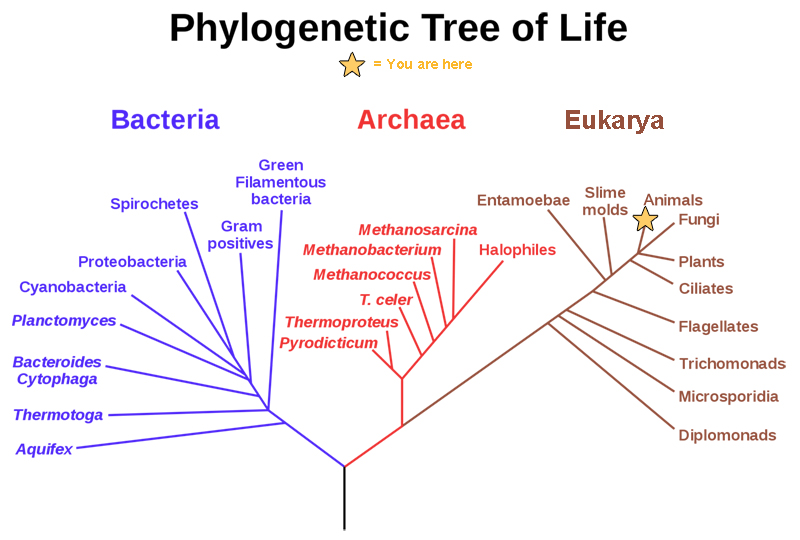
\includegraphics[width=\textwidth]{./img/phylogenetic_tree.jpg}
		\caption{Теоретически укоренённое филогенетическое дерево, показывающее общее происхождение организмов из всех трёх доменов: Бактерии, Археи, Эукариоты.}
	\end{figure}
	\subsection{Анализ сетей биологических взаимодействий}
	\subsection{Конструирование интегральных схем}
	\section{Доказательство NP-полноты задачи}
	\begin{theorem}
		$$ \{ (G, k)\ |\ \text{ в неориентированном графе G есть дерево Штейнера веса } \le k \in \Integer \} \in \mathrm{NPC} $$
	\end{theorem}
	\begin{proof}$  $
		\begin{enumerate}
			\item \textbf{STEINER-TREE $\in$ NP}: 
				Сертификат должен проверять, что поданный ему на вход подграф $T$ является деревом, содержит все терминальные вершины и имеет вес $\le k$, причём вторая и третья подзадачи тривиальны. Согласно одному из эквивалентных определений дерева, достаточно проверить связность $T$ и то, что $|E(T)| = |V(T)| - 1$, для чего достаточно обхода в глубину. Т.е. полиномиальный сертификат существует и STEINER-TREE $\in$ NP.
			\item \textbf{VERTEX-COVER $\le_{p}$ STEINER-TREE}: Полиномиальное сведение устроено так:
			\begin{enumerate}
				\item Дополним $G$ до $K_{|V|}$, где каждое ребро поделим на 2 и назовём результат $G' = (V', E')$.
				\begin{gather*}
					W := \{ w_i\ |\ e_i = (u, v) \in E \implies (u, w_i), (w_i, v) \in E' \}\\
					V' = V \cup W\\
					\begin{aligned}
						E' = V^2 \cup \{& (u, w) \in V \times W\ |\\
						&\exists v \in V: (u, w), (w, v) \in E' \}
					\end{aligned}
				\end{gather*} 
				\item Если $\forall e' \in E': w'(e') = 1$ и $V_0' = W$, то в $G'$ есть дерево Штейнера веса не более $|E| + k - 1 \iff $ в $G$ есть вершинное покрытие мощности $\le k$.
			\end{enumerate}
			\begin{proof}$  $
				\begin{itemize}
					\item $ \underline{\implies} $: Пусть $T$ — дерево Штейнера для $V_0'$ в $G'$, тогда $C := V(T) \setminus V_0'$ — вершинное покрытие в $G$: $ V(T) \setminus V_0' \subset V$ и накрывает каждое ребро $e \in E$ по построению. $ |C| = |V(T)| - |V_0'| = \omega(T) + 1 - |V_0'| \le (|E| + k - 1) + 1 - |V_0'| = k$, т.к. $|E| = |V_0'|$. 
					\item $ \underline{\impliedby} $:  Пусть $C \subset V$ — вершинное покрытие, $|C| \le k$, $T$ — дерево на вершинах $C$ в $G'$.\footnote{Такое дерево всегда существует, т.к. $V^2 \subset V(G')$.} Чтобы гарантировать $V_0' \subset V(T)$, для каждой вершины $v_0' \in V_0' \setminus V(T)$ добавим в $T$ ребро $(v_0', c)$, где $c \in C$ — вершина покрытия, накрывающая ребро, подразделением которого получена $v_0'$. Полученный граф содержит $\le |E| + |C| - 1 \le |E| + k - 1$ рёбер. Если в процессе расширения в $T$ образовались циклы, их можно раскрыть, уменьшив суммарный вес. По завершении получим дерево Штейнера веса $\le |E| + k - 1$ в $G'$.
				\end{itemize} 
			\end{proof}
			Все шаги построения $G'$ полиномиальны: добавляется $O(|V|^2)$ рёбер и вершин. Для восстановления вершинного покрытия по дереву Штейнера в $G'$ нужно брать разность множеств — $O(|V|^2)$ операций, а в обратную сторону нужно перебрать $V_0'$ и исходящие из него рёбра (не более двух на каждую вершину) — тоже $O(|V|^2)$ операций. Следовательно, сведение полиномиально, а его корректность была доказана выше.
		\end{enumerate}
	\end{proof}
	\section{Сведение к метрическому случаю}
		Часто хочется потребовать, чтобы для весовой функции выполнялось правило треугольника:
		$$
			\omega(x, y) \le \omega(x, z) + \omega(z, y) 		
		$$
		причём она должна быть определена на $V^2$. Такая весовая функция играет роль метрики на множестве вершин и становится проще для восприятия. В таком случае говорят о поиске \textit{метрического} дерева Штейнера, и именно такой вид задачи был исторически первым.
		\begin{preposition}$  $
			\begin{enumerate}
				\item Существует полиномиальное сведение задачи о дереве Штейнера к метрическому случаю.
				\item Оптимальные ответы к обеим задачам совпадают.
			\end{enumerate}
		\end{preposition}
		\begin{proof}
			Предложенная конструкция основана на понятии \textit{метрического замыкания}:
			\begin{definition}
				Пусть $ G = (V, E, \omega) $ — неориентированный взвешенный граф, $d: V^2 \to \Real^{+} $ — функция расстояния, сопоставляющая паре вершин длину кратчайшего пути между ними. Тогда граф $G'$, построенный по следующим правилам, называется \textit{метрическим замыканием} графа $G$:
				$$
					G' = (V, E', d),\ E' = \{ (u, v, d(u, v))\ |\ u, v \in V,\ u \neq v \}
				$$
				Полученный граф является метрическим, т.к. для $d$ выполнено правило треугольника: если $ d(x, y) > d(x, z) + d(z, y) $, то путь $x \to y$ можно было бы прорелаксировать конкатенацией путей $x \to z$ и $z \to y$, что противоречит определению $d(x, y)$ как длины \textit{кратчайшего} пути $x \to y$.\\
				Построить метрическое замыкание можно за $O(|V|^3)$ алгоритмом Флойда-Уоршелла. 
			\end{definition}
			\noindent Пусть $T, T'$ — деревья Штейнера для $V_0$ в $ G $ и $ G' $ соответственно. Докажем, что $\omega(T) = d(T')$. Очевидно, что $ d(T') \le \omega(T) $, т.к. переход к кратчайшим путям не ухудшает ответ. Более того, каждое ребро в $T'$ можно "разжать" в тот кратчайший путь, из которого он был получен, после чего выбрать в полученном графе минимальное остовное дерево $T''$. $\omega(T'') \le d(T')$, т.к. теперь каждое ребро встречается ровно один раз, а ранее могло вносить свой вклад одновременно в несколько кратчайших путей. Но $T''$ по построению — дерево Штейнера для $V_0$ в $G$! Следовательно, $ \omega(T) = \omega(T'') \le d(T') \le \omega(T)$, т.е. $\omega(T) = d(T')$.
 		\end{proof}
	\section{2-оптимальный алгоритм}
	\begin{theorem}$  $\\
		Существует 2-оптимальный алгоритм для метрического случая задачи поиска дерева Штейнера:
		\begin{enumerate}
			\item Считать граф $G = (V, E, \omega)$ и множество терминальных вершин $V_0$.
			\item Построить метрическое замыкание $G' = (V, E', d)$ графа $G$.
			\item Выделить $H'$ — подграф в $G'$, индуцированный вершинами $V_0$. 
			\item Построить минимальное остовное дерево $T_{\mathrm{MST}}$ в $H'$.
			\item Вернуть полученный $T_{\mathrm{MST}} $ в качестве ответа.
		\end{enumerate}
	\end{theorem}
	\begin{proof}
		Пусть $T_{S}$ — дерево Штейнера для $V_0$ в $G'$.\\
		Вершины $T_{S}$ в порядке обхода в глубину
		$$
			u_0, u_1, \ldots, u_m = u_0
		$$ 
		задают Эйлеров цикл, потому:
		$$ 
			\sum_{i=0}^{m-1} d(u_i, u_{i+1}) = 2 \cdot d(T_{S})
		$$
		Если исключить из рассмотрения все нетерминальные вершины и оставить только первое вхождение всех терминальных, то получим путь:
		$$
			v_0, v_1, \ldots, v_k
		$$
		содержащий все терминальные вершины (т.к. изначально это был обход $G'$).\\ 
		По неравенству треугольника:
		$$
			d(v_i, v_{i+1}) \le \sum_{j=1}^{t} d(u_{i_j}, u_{i_{j+1}})
		$$
		Здесь $v_{i_{j}}, \ldots, v_{i_{t+1}}$ - последовательные вершины в обходе в глубину, причём $v_i = u_{i_{1}}, u_{i+1} = v_{i_{t+1}}$.\\
		Поскольку $y_1, \ldots, y_k$ — путь, это также дерево, причём неравенство треугольника гарантирует, что добавление любой вершины только увеличивает его вес. Более того, в силу того, как задана весовая функция, это ещё и минимальное остовное дерево в $H'$. Следовательно, это дерево Штейнера $T_{\mathrm{MST}}$ для $V_0$ в $G'$, причём:
		\begin{gather*}
			d(T_{\mathrm{MST}}) \le \sum_{i=1}^{n} d(u_i, u_{i+1}) = 2 \cdot d(T_{S})\\
			1 \le \frac{d(T_{\mathrm{MST}})}{d(T_{S})} \le 2
		\end{gather*}
		По \textit{утверждению 3.1.}, по нему восстанавливается дерево Штейнера в $G$.
	\end{proof}
	\clearpage
	\begin{figure}[!hbtp]
	\centering
	\begin{tikzpicture}
		\pgfmathsetmacro{\n}{7}
		\node[draw=none,minimum size=6cm,regular     polygon,regular polygon sides=\n] (poly) {};
		\begin{scope}[every node/.style={circle,thick,draw}]
			\fill[black] (0, 0) circle[radius=4pt];
			\foreach \x in {1,2,...,\n} {
				\fill[red] (poly.corner \x) circle[radius=4pt];
			}
		\end{scope}
		\begin{scope}[>={Stealth[black]},
			every node/.style={fill=white,circle},
			every edge/.style={draw=blue,thick}]
			 \foreach \x in {1,2,...,\n} {
		 		\path[->] (0, 0) edge node {$1$} (poly.corner \x);
			 }
		\end{scope}
		\begin{scope}[>={Stealth[black]},
			every node/.style={fill=white,circle},
			every edge/.style={draw=red,thick}]
			\foreach \x in {1,2,...,\n} {
				\pgfmathtruncatemacro{\cur}{\x};
				\pgfmathtruncatemacro{\next}{max(1, Mod(\cur + 1, \n + 1)};
				\path[->] (poly.corner \cur) edge node {$2$} (poly.corner \next);
			}
		\end{scope}
		\begin{scope}[>={Stealth[black]},
			every node/.style={fill=white,circle},
			every edge/.style={draw=black,thick}]
				\path[->] (poly.corner \n) edge node {$2$} (poly.corner 1);
		\end{scope}
	\end{tikzpicture}
		\caption{  Пример графа, на котором оценка достигается (в пределе). Терминальные вершины выделены красным. Реальное дерево Штейнера $ T_{S} $ выделено синим, а $ T_{\mathrm{MST}} $, построенное алгоритмом, — красным. Если внешний цикл имеет вид $n$-угольника, то верно, что $ \frac{d(T_{\mathrm{MST}})}{d(T_{S})} = \frac{2n-2}{n} = 2 - \frac{2}{n} \to 2 $. } 
	\end{figure}
	\section{Реализация}
	\subsection{Асимптотика работы алгоритма и ограничения по его применению}
	\begin{enumerate}
		\item Алгоритм Флойда-Уоршалла поиска кратчайших путей между всеми парами вершин: $\Theta(|V|^3)$ операций, $ \Theta(|V|^2) $ памяти на хранение матрицы расстояний. 
		\item Алгоритм Краскала поиска минимального остовного дерева с помощью системы непересекающихся множеств: $O(|E| \log |V|)$ операций, $ \Theta(|V|) $ памяти. 
	\end{enumerate}
	Т.к. метрическое замыкание делает граф полным, итого имеем $ \Theta(|V|^3) $ операций и $\Theta(|V|^2)$ памяти. Следовательно, алгоритм оправданно применять при $ |V| \le 1000 $, что является существенным недостатком предложенного подхода.\\
	
	\noindent Также стоит отметить, что алгоритмы Флойда-Уоршалла и Краскала по своей природе последовательные, в связи с чем воспользоваться преимуществами вычислительного кластера МФТИ, к которому автор имеет авторизованный доступ, не представляется возможным при таком подходе.\\
	
	\noindent Более того, алгоритм Флойда-Уоршалла хорош тем, что не совершает больших прыжков по памяти при хранении матрицы кратчайших расстояний в виде последовательно расположенной в памяти двумерной таблицы, что уменьшает число промахов по кэшу процессора и оказывает положительный эффект на скорость работы алгоритма по сравнению с параллельными запусками алгоритмов поиска кратчайших путей из данной вершины во все остальные (в духе алгоритма Дейкстры) при малых $|V|$.\\
	
	\noindent Тем не менее, при $|V| \ge 10^3$ не лишено смысла хранить исходную матрицу расстояний в базе данных (на жёстком диске или распределённо) и действительно выполнять параллельные запуски, скажем, алгоритма Дейкстры на доступных процессорах для параллельного подсчёта матрицы кратчайших расстояний. Эта неасимптотическая оптимизация делает возможной обработку существенно б\textbf{о}льших графов, чем было заявлено изначально, т.к. это типичная map-reduce задача, что с точки зрения автора является довольно дешёвой в реализации, но полезной идеей, пусть и выходящей за рамки требований поставленной учебной задачи. 
	
	\subsection{Использованные технологии}
			Для работы с графами в Python была использована библиотека \href{https://graph-tool.skewed.de/static/doc/topology.html#graph_tool.topology.shortest_distance}{graph-tool}. По опыту автора, альтернативы в лице \href{https://networkx.github.io/}{networkx} и \href{https://igraph.org/python/}{igraph} имеют слишком много нетривиальных недостатков: networkx написана на Pure Python, из-за чего производительность становится неприемлемой уже на маленьких графах, а разработка Python-API для написанной на C библиотеки igraph уже больше года как приостановлена, а по состоянию на данный момент пользоваться ей очень уж неудобно по причинам, расписывать которые слишком долго для того, чтобы приводить их здесь. R-API гораздо лучше, но Python для меня предпочтительнее.
	\subsection{Проверка корректности}
		Тесты разделены на несколько групп:
		\begin{enumerate}
			\item Маленькие ($|V| \le 20$) случайные графы в модели Эрдеша-Рейни, реальное дерево Штейнера в которых ищется полным перебором (возможно, с некоторыми эвристиками).
			\item В качестве примера реальной задачи рассматривается поиск дерева Штейнера на географической карте города, где некоторые строения помечены и играют роль терминальных вершин. Данные взяты из \href{https://homepage.univie.ac.at/ivana.ljubic/research/STP/}{Принстонской статьи}, но вынужденно ограничены до 1000 точек на карте в силу кубической асимптотики алгоритма.
		\end{enumerate}
	\section{Список литературы}
\end{document}     